%!TEX root = IntensionalSemantics.tex
\chapter{Conditionals: The Restrictor Theory}\label{cha:conditionals-restrictor} % (fold)

\chapterprecishere{We look at the interaction of conditionals with modals and find that we need a better theory of \emph{if}-clauses.}

\minitoc

We now have a basic theory of conditionals in place as well as a basic theory of modals. Both are treated as intensional operators that move us from the initial evaluation world to another set of worlds: in the case of conditionals, those worlds where the antecedent is true that are otherwise relevantly like the evaluation world; in the case of modals, to whatever worlds the contextually supplied accessibility relation assigns to the evaluation world.

\section{The interaction of conditionals and modals}

This means that if a sentence contains both a conditional and a modal, we expect them to work together to express nested intensional shifting, very much like our analysis of the sentence \emph{you might have to leave} in the previous chapter.

Consider then the following sentence:

\ex. \label{ex:lockhart-must}If we are on Route 183, we must be in Lockhart.

Imagine two friends on a road trip. They have lost all their electronic devices that might have had GPS functionality. They are lost, except that they have an old-fashioned map with them. Here's a schematic representation of the relevant geographical area:

% \begin{wrapfigure}{l}{40mm}
%   \begin{center}
    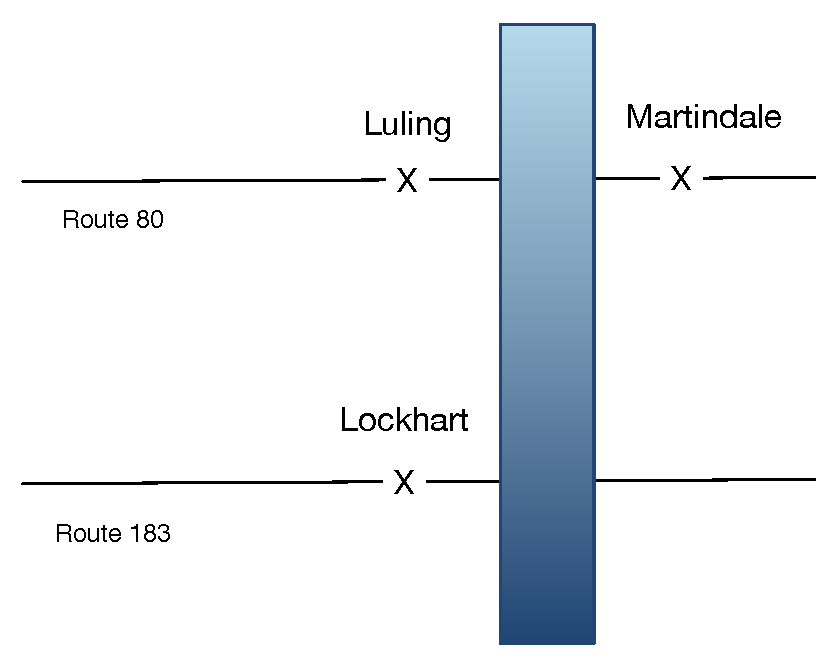
\includegraphics[width=\textwidth]{183new}
%   \end{center}
%   \caption{A schematic map of the relevant area}
% \end{wrapfigure}

Our friends are lost. They might be on Route 80 or they might be on Route 183. They come to a river. They do not know which direction they're facing (it's high noon in Texas). They determine that they are in one of three towns: Lockhart, Luling, or Martindale. One of them says \Last. That seems true.

Let's consider what our semantics predicts.

\begin{exercise}
Calculate the truth-conditions of \Last with respect to an arbitrary world $w$,
and assignment function $g$. Assume that \emph{must} scopes over \emph{we be in Lockhart}. Do not worry about the internal composition of the two embedded clauses.

Assume the following lexical entries for \emph{if} and \emph{must}:

$\svwg{if} = \lambda p_{st}.\lambda q_{st}.\ \forall w'\co p(w') = 1\ \&\ w'
\text{ relevantly like } w \rightarrow q(w') = 1$

$\svwg{must} = \lambda p_{st}.\ \forall w' \text{ compatible with the evidence
  in } w\co p(w') = 1$ \eex
\end{exercise}
%
The prediction is that the conditional takes us to worlds where our friends are on Route 183 and that are otherwise like the evaluation world. The modal then looks at the evidence in those Route 183 worlds and says that in all worlds compatible with that evidence, they are in Lockhart. 

This is wrong: no matter whether they are on Route 183 or on Route 80, our friends are lost. So, their evidence in any of the relevant worlds is the same: inconclusive as to where they are. In none of the worlds do they have evidence about which of the three possible towns they are in. Thus, our semantics incorrectly predicts that \Last is false in the given scenario. But it is clearly true.

\section{\expression{If}-Clauses as Restrictors}

The problem we have encountered here with the interaction of an \expression{if}-clause and the modal operator \expression{might} is similar to others that have been noted in the literature. Most influentially, David Lewis in his paper ``Adverbs of Quantification'' showed how hard it is to find an adequate analysis of the interaction of \expression{if}-clauses and \term{adverbs of quantification} like \expression{never, rarely, sometimes, often, usually, always}. Lewis proposed that in the cases he was considering, the adverb is the only operator at work and that the \expression{if}-clause serves to restrict the adverb. Thus, it has much the same function that a common noun phrase has in a determiner-quantification. %\marginpar{\centering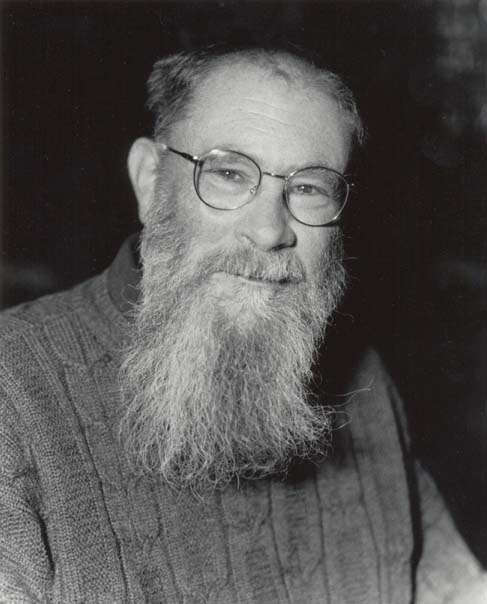
\includegraphics[height=1in]{lewis.jpg}\\ {\tiny \href{http://en.wikipedia.org/wiki/David_Lewis_(philosopher)}{David Lewis}}}

\begin{quote}
	
	The \expression{if} of our restrictive \expression{if}-clauses should not be regarded as a sentential connective. It has no meaning apart from the adverb it restricts. The \expression{if} in \expression{always if \ldots, \ldots, sometimes if \ldots, \ldots}, and the rest is on a par with the non-connective \expression{and} in \expression{between \ldots and \ldots}, with the non-connective \expression{or} in \expression{whether \ldots or \ldots}, or with the non-connective \expression{if} in \expression{the probability that \ldots if \ldots}. It serves merely to mark an argument-place in a polyadic construction. \cite[11]{lewis:1975:adverbs}

\end{quote}
%
Building on Lewis' insight, Kratzer argued for a uniform treatment of \expression{if}-clauses as restrictors. She claimed that 

\begin{quote}
	
	the history of the conditional is the story of a syntactic mistake. There is no two-place \expression{if \ldots then} connective in the logical forms of natural languages. \expression{If}-clauses are devices for restricting the domains of various operators. \citep{kratzer:1986:conditionals}
\end{quote}
%
Let us repeat this:

\ex. \extitle{Kratzer's Thesis}\\[3pt]
\expression{If}-clauses are devices for restricting the domains of various operators.

Kratzer's Thesis gives a unified picture of the semantics of conditional clauses. Note that it is not meant to supplant previous accounts of the meaning of conditionals. It just says that what those accounts are analyzing is not the meaning of \expression{if} itself but the meaning of the operators that \expression{if}-clauses restrict. 

Let us see how this idea helps us with our Lockhart-sentence. The idea is to deny that there are two quantifiers over worlds in \ref{ex:lockhart-must}. Instead, the \expression{if}-clause merely contributes a further restriction to the modal \expression{might}. In effect, the modal is not quantifying over \emph{all} the worlds compatible with Mary's knowledge but only over those where they are on Route 183. It then claims that at least some of those worlds are worlds where they are in Lockhart. We cannot anymore derive the problematic conclusion that it should also be true that if they are on the Route 80, they might be in Lockhart. In all, we have a good analysis of what \ref{ex:lockhart-must} means.

What 
%
\marginpar{
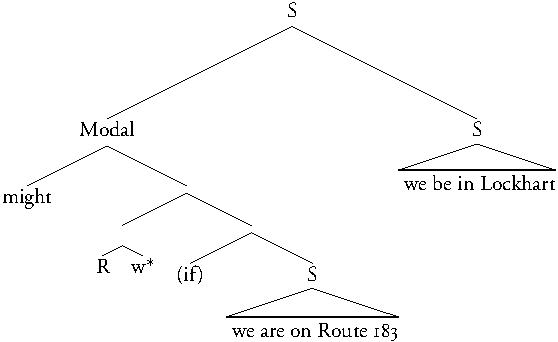
\includegraphics[width=\marginparwidth]{lockhartlf-final}\figcaption{LF for \ref{ex:lockhart-must}}}
%
we don't yet have is a compositional calculation. What does it mean in structural terms for the \expression{if}-clause to be restricting the domain of the modal? We will assume a structure as in the LF in the margin. Here, the \expression{if}-clause is the sister to what used to be the covert set-of-worlds argument of the modal. As you can see, we have chosen the variant of the semantics for modals that was discussed in Section \ref{techvariant}. The idea now is that the two restrictive devices work together: we just feed to the modal the \emph{intersection} of (i) the set of worlds that are $R$-accessible from the actual world, and (ii) the set of worlds where they are on Route 183.

\begin{exercise}
	
	To make the composition work, we need to be able to intersect the set of accessible worlds with the antecedent proposition. This could be done in two ways: (i) a new composition principle, which would be a slight modification of the \term{Predicate Modification} rule, (ii) give \expression{if} a functional meaning that accomplishes the intersection. Formulate such a meaning for \expression{if}.
	
	Alternatively, we could do without the $w*$ device and instead give \expression{if} a meaning that takes a proposition $p$ and then modifies an accessibility relation to give a new accessibility relation, which is restricted to $p$-worlds. Formulate such a meaning for \expression{if}. 

Finally, we could rethink the LF and treat the \emph{if}-clause as a direct sister of the modal. Devise a meaning for \emph{if} that would give the right meaning for \ref{ex:lockhart-must}.\eex
\end{exercise}

What about cases like the earthquake conditional from Chapter 2, now? 

\ex. If there's an earthquake, my house will collapse.

Here there is no modal operator for the \expression{if}-clause to restrict. Should we revert to treating \expression{if} as an operator on its own? Kratzer proposes that we should not and that such cases simply involve covert modal operators. % We will have nothing to say about that here.

%\bigskip\noindent [MUCH MORE TO COME \dots]

\newpage\section*{Supplementary Readings} \label{sec:suppl-read-conditionals}

\phantomsection \addcontentsline{toc}{section}{Supplemental Readings}

{\setlength{\parindent}{0pt}\setlength{\parskip}{6pt}

A short handbook article on conditionals:
\begin{bibentrylist}
	\item\bibentry{fintel:2009:hsk-conditionals}.
\end{bibentrylist}

Overviews of the philosophical work on conditionals:
\begin{bibentrylist}
	\item \bibentry{edgington:1995:conditionals}.
	\item \bibentry{bennett:2003:guide}.
\end{bibentrylist}

A handbook article on the logic of conditionals:
\begin{bibentrylist}
	\item \bibentry{nute:1984:conditional}.
\end{bibentrylist}

Three indispensable classics:
\begin{bibentrylist}
	\item \bibentry{lewis:1973:counterfactuals}.
	\item \bibentry{stalnaker:1968:theory}.
	\item \bibentry{stalnaker:1975:indicative}. 
\end{bibentrylist}

The Restrictor Analysis:
\begin{bibentrylist}
	\item \bibentry{lewis:1975:adverbs}. 
	\item \bibentry{kratzer:1986:conditionals}.
\end{bibentrylist}

The application of the restrictor analysis to the interaction of nominal quantifiers and conditionals:
\begin{bibentrylist}
	\item \bibentry{fintel:1998:qandif}.
	\item \bibentry{fintel-iatridou:2002:ifwhen}.
	\item \bibentry{higginbotham:2003:conditionals}.
	\item \bibentry{leslie:2009:unless}.
	\item \bibentry{huitink:2009:quantified-conditionals}.
\end{bibentrylist}

Syntax of conditionals:
\begin{bibentrylist}
  \item \bibentry{fintel:1994:thesis}, Chapter 3: ``Conditional Restrictors''
  \item \bibentry{iatridou:1993:then}.
	\item \bibentry{bhatt-pancheva:2006:conditionals}.
\end{bibentrylist}

A shifty alternative to the restrictor analysis:

\begin{bibentrylist}
  \item \bibentry{gillies:2009:truth-conditions}.
  \item \bibentry{gillies:2010:iffiness}.
\end{bibentrylist}

The Belnap alternative:

\begin{bibentrylist}
   \item \bibentry{belnap:1970:restricted}.
   \item \bibentry{belnap:1973:restricted}.
   \item \bibentry{fintel:2007:gurt-slides}.
   \item \bibentry{huitink:2008:thesis}, Chapters 1 and 2 give a nice summary of what we're covering in this class, while Chapter 5 is about the Belnap-method.
   \item \bibentry{huitink:2009:domain-conditionals}.
\end{bibentrylist}
  
}

% chapter conditionals (end)

